\documentclass[12pt,a4paper,oneside,ngerman]{article} 
\usepackage[left=3cm,right=3cm,top=2.5cm]{geometry} % Groesse der Seitenraender definieren
\usepackage[utf8]{inputenc} % utf8 encoding
\usepackage{hyperref}
\usepackage{ngerman}
\usepackage{graphicx}
\usepackage{tikz} % Automaten, Graphen, ... zeichnen
\usepackage{tikz-qtree} % Paket fuer Tikz Graphen-Baeume
\usetikzlibrary{arrows,shapes,automata} % Bestimmte tikz-Befehle benutzen
\usepackage{amsmath,amssymb} % Mathe-Formeln und -Ausdruecke
\usepackage{listings} % Code-Ausschnitte einbinden
\usepackage{xcolor} % Eigene Farben definieren
\usepackage{colortbl} % Farben verwenden in Tabellen
\usepackage{wrapfig} % Bilder von Text umfliessen lassen
\usepackage{multicol} % Mehrspaltigen Text schreiben
\usepackage{stmaryrd} % Fuer Symbole wie zu Beispiel Widerspruchspfeil
\usepackage{caption}
\usepackage{totpages}

\usepackage{circuitikz}
\usepackage{amsmath}
\usepackage{graphicx}
\usepackage{subfigure}
\usepackage{tikz}

% Beliebige RGB Farben definieren:
\definecolor{gold}{rgb}{0.83, 0.69, 0.15}
\definecolor{magenta}{rgb}{0.79, 0.08, 0.48}

% Titel in Kopfzeilen
\usepackage{fancyhdr}
\pagestyle{fancy}
\fancyhf{}
\setlength{\headheight}{20pt}

% Seitenumbrueche werden nicht mehr eingerueckt
\setlength{\parindent}{0em}


% % % % % % % % % % % % % % % % % % % % % % % % % % % % % % 
%Variablen
% % % % % % % % % % % % % % % % % % % % % % % % % % % % % % 
\newcommand{\fach}{Objektorientierte Modellierung und Programmierung}
\newcommand{\dokumentenTitel}{Abgabe Uebungsblatt Nr.02}
\newcommand{\Abgabe}{05.05.2020, 12:00 Uhr}
\newcommand{\memberOne}{Marius Birk}
\newcommand{\memberTwo}{Pieter Vogt}


\newcommand{\tutor}{ Florian Brandt }
% % % % % % % % % % % % % % % % % % % % % % % % % % % % % 

% Kopfzeile auf jeder Seite:
\fancyhead[R]{\dokumentenTitel} % Dokument-Titel
\fancyhead[C]{}
\fancyhead[L]{\memberOne, \memberTwo} % Autorennamen
\renewcommand{\headrulewidth}{0.4pt} %obere Trennlinie

% Fußzeile auf jeder Seite:
\fancyfoot[C]{Seite \thepage \ von \ref{TotPages}} %Seitennummer
\renewcommand{\footrulewidth}{0.4pt} %untere Trennlinie

% Nun beginnt das eigentliche Dokument
\begin{document}
	\thispagestyle{plain} % Keine Kopfzeile auf erster Seite, aber Seitenzahl wird angezeigt
	
	\begin{multicols}{2} % Beginnt zweispaltigen Text fuer Header auf erster Seite
		\hspace{-1cm} % Linken Header-Teil 1cm nach links schieben.
		% Tabelle fuer linke Seite vom Header der ersten Seite
		\begin{tabular}{ll} % Mit l werden die Eintraege linksbuendig
			Autoren: & \memberOne \\ % Zwischen jeder Spalte ein & einfuegen
			& \memberTwo \\
% beendet eine Tabellenzeile 
			Tutor: & \tutor \\  
		\end{tabular}
		
		\columnbreak % Nun beginnt die rechte Seite des Headers
		\hspace{-1cm} % Rechten Header-Teil 1cm nach links schieben.
		% Tabelle fuer rechte Seite vom Header der ersten Seite
		\begin{tabular}{ll} % p{1cm} bewirkt, dass die rechte Spalte 6cm breit ist.
			Abgabe: & \Abgabe \\ % Zwischen jeder Spalte ein & einfuege
			Smileys: &  
			%Mit diesem Befehl wird die Zeilenhoehe der folgenden Tabelle um 20% erhoeht.   
			\renewcommand{\arraystretch}{1.2} 
			% Nun kommt eine innere Tabelle in der aeusseren Tabelle, mit der eine Punktetabelle fuer den Tutor erstellt wird:  
			\begin{tabular}{|p{0.8cm}|p{0.8cm}|p{0.8cm}|p{0.8cm}|}
				\hline A1 & A2 & A3 & $\sum\limits^{ }$ \\ \hline
				& & & \\ \hline    
			\end{tabular} \\
		\end{tabular}
		
	\end{multicols} % Beendet zweispaltigen Text
	
	\begin{center}
		\Large{\fach} \\
		\LARGE{\dokumentenTitel} \\
		\small
		$($Alle allgemeinen Definitionen aus der Vorlesung haben in diesem Dokument bestand, es sei den sie erhalten eine explizit andere Definition.$)$
    \end{center}

		\begin{figure}[h]
			Tenis
			\section{Aufgabe 1}

			\subfigure[Klassendiagramm Star, StarsDatabase]{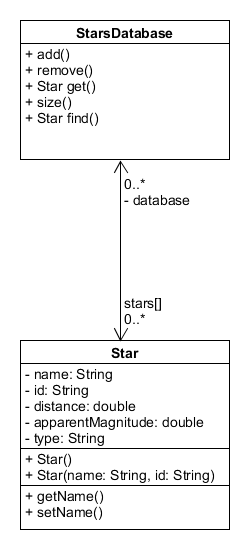
\includegraphics[width=0.2\textwidth]{Von Pieter/Klassendiagramm Sternendatenbank}}
			\subfigure[Objektdiagramm Sirius]{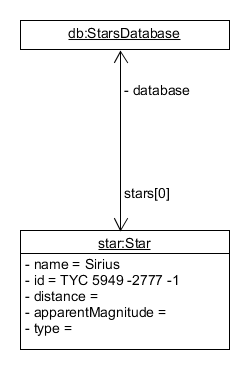
\includegraphics[width=0.3\textwidth]{Von Pieter/Objektdiagramm Test1 Sternendatenbank}}
			\subfigure[Objektdiagramm Sirius, Alpha Centauri]{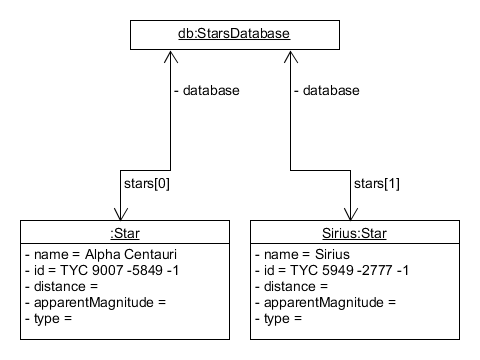
\includegraphics[width=0.4\textwidth]{Von Pieter/Objektdiagramm Test2 Sternendatenbank}}
			\subfigure[Objektdiagramm Alpha Centauri, Sirius]{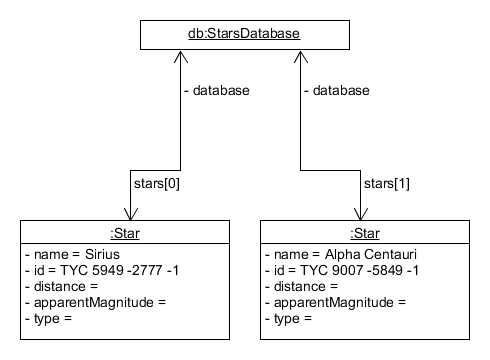
\includegraphics[width=0.4\textwidth]{Von Pieter/Objektdiagramm Test3 Sternendatenbank}}
		\end{figure}
	\newpage
    \section{Aufgabe 2}
        \subsection{a)}
            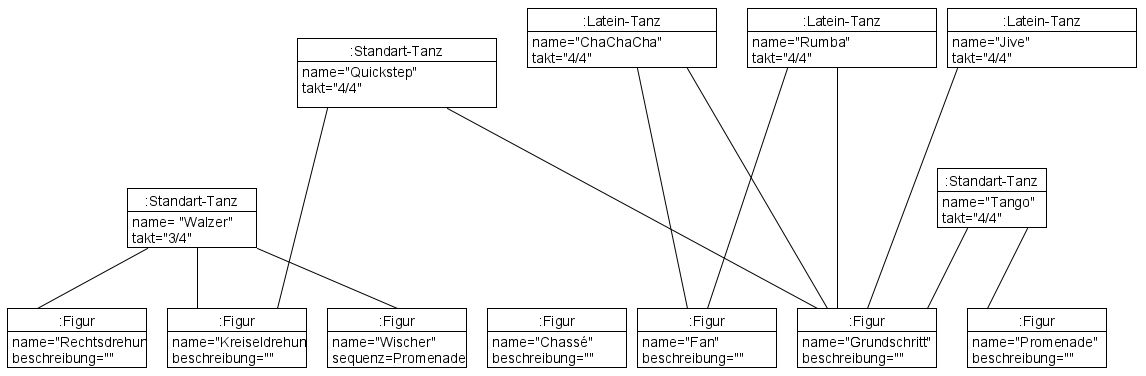
\includegraphics[width=18cm]{Objektdiagramm A_2}\\\\
        \subsection{b)}
                \subsubsection{Dance Code}
                    \begin{verbatim}
						import java.util.ArrayList;

						class Dance {
							private String name;
							private String beat;
							private ArrayList figures = new ArrayList();
						
							public void getFigures() {
								System.out.println(this.figures);
						
							}
						
							public void setFigures(String Figures) {
								this.figures.add(Figures);
							}
						
							public String getName() {
								return name;
							}
						
							public void setName(String name) {
								this.name = name;
							}
						
							public String getBeat() {
								return beat;
							}
						
							public void setBeat(String beat) {
								this.beat = beat;
							}
						
						}
						
						class StandardDance extends Dance {
						
						}
						
						class LatinDance extends Dance {
						
						}
						
						class Figure {
							private String name;
							private String text;
						
							public String getName() {
								return name;
							}
						
							public void setName(String name) {
								this.name = name;
							}
						
							public String getText() {
								return text;
							}
						
							public void setText(String text) {
								this.text = text;
							}
						
						}
						
						class Sequence extends Figure {
							public ArrayList<String> figures = new ArrayList<String>();
						
							public void setSequence(ArrayList sequence) {
								this.figures = sequence;
							}
						
							public boolean add(String figure) {
								if (figures.contains(figure)) {
									return false;
								} else {
									figures.add(figure);
									return true;
								}
							}
						}
					\end{verbatim}
				\subsubsection{Dance Database}
					\begin{verbatim}
						import java.io.FileReader;
						import java.util.ArrayList;

						public class DanceDatabase {
							public static void main(String[] args) {
								ArrayList<String> Figures = new ArrayList<String>();
								Figures.add("Rightturn");
								Figures.add("Basic Movement");
								Figures.add("Spin Turn");
								Figures.add("Promenade");
								Figures.add("Chasse");
								Figures.add("Fan");
								Figures.add("Whisk");
						
								Sequence S_Whisk = new Sequence();
								if (S_Whisk.add("Chasse")) {
									System.out.println("Hinzufügen erfolgreich");
									//Um diese Prüfung zu realisieren musste das Objekt Array auf eine Object ArrayList geändert werden, in dem die Figuren
									//gespeichert werden.
								} else {
									System.out.println("Hinzufügen nicht erfolgreich");
								}
								if (S_Whisk.add("Promenade")) {
									System.out.println("Hinzufügen erfolgreich");
									//Um diese Prüfung zu realisieren musste das Objekt Array auf eine Object ArrayList geändert werden, in dem die Figuren
									//gespeichert werden.
								} else {
									System.out.println("Hinzufügen nicht erfolgreich");
								}
								StandardDance Walzer = new StandardDance();
								Walzer.setName("Walzer");
								Walzer.setBeat("3/4");
								Walzer.setFigures(Figures.get(0));
								Walzer.setFigures(Figures.get(2));
								Walzer.setFigures(Figures.get(6));
						
								StandardDance Tango = new StandardDance();
								Tango.setBeat("4/4");
								Tango.setName("Tango");
								Tango.setFigures(Figures.get(1));
								Tango.setFigures(Figures.get(3));
						
								StandardDance Quickstep = new StandardDance();
								Quickstep.setBeat("4/4");
								Quickstep.setName("Quickstep");
								Quickstep.setFigures(Figures.get(1));
								Quickstep.setFigures(Figures.get(2));
						
								LatinDance Cha = new LatinDance();
								Cha.setBeat("4/4");
								Cha.setName("ChaChaCha");
								Cha.setFigures(Figures.get(1));
								Cha.setFigures(Figures.get(5));
						
								LatinDance Rumba = new LatinDance();
								Rumba.setBeat("4/4");
								Rumba.setName("Rumba");
								Rumba.setFigures(Figures.get(1));
								Rumba.setFigures(Figures.get(5));
						
								LatinDance Jive = new LatinDance();
								Jive.setBeat("4/4");
								Jive.setName("ChaChaCha");
								Jive.setFigures(Figures.get(1));
							}
						
						}

					\end{verbatim}
			\subsection{c)}
			\begin{verbatim}
				public boolean add(String figure) {
					if (figures.contains(figure)) {
						return false;
					} else {
						figures.add(figure);
						return true;
					}
				}
			\end{verbatim}
	\section{Aufgabe 3}
			\subsection{a)}
			\begin{verbatim}
				public class Out {
    public void out(String s){
        System.out.println(s);
    }
    public void out(boolean b){
        System.out.println(b);
    }
    public void out(int i){
        System.out.println(i);
    }
    public void out(double d){
        System.out.println(d);
    }
    public void out(char c){
        System.out.println(c);
    }

    public void out(Object o){
        System.out.println(o);
    }
}
			\end{verbatim}
\end{document}
